\section{外设与中断}

\subsection{概述}

我们在外设方面实现了作为输出设备的屏幕以及输入设备的键盘,在中断方面同时实现了硬件中断与软件中断。

\subsubsection{VGA像素映射的屏幕}

\begin{center}
    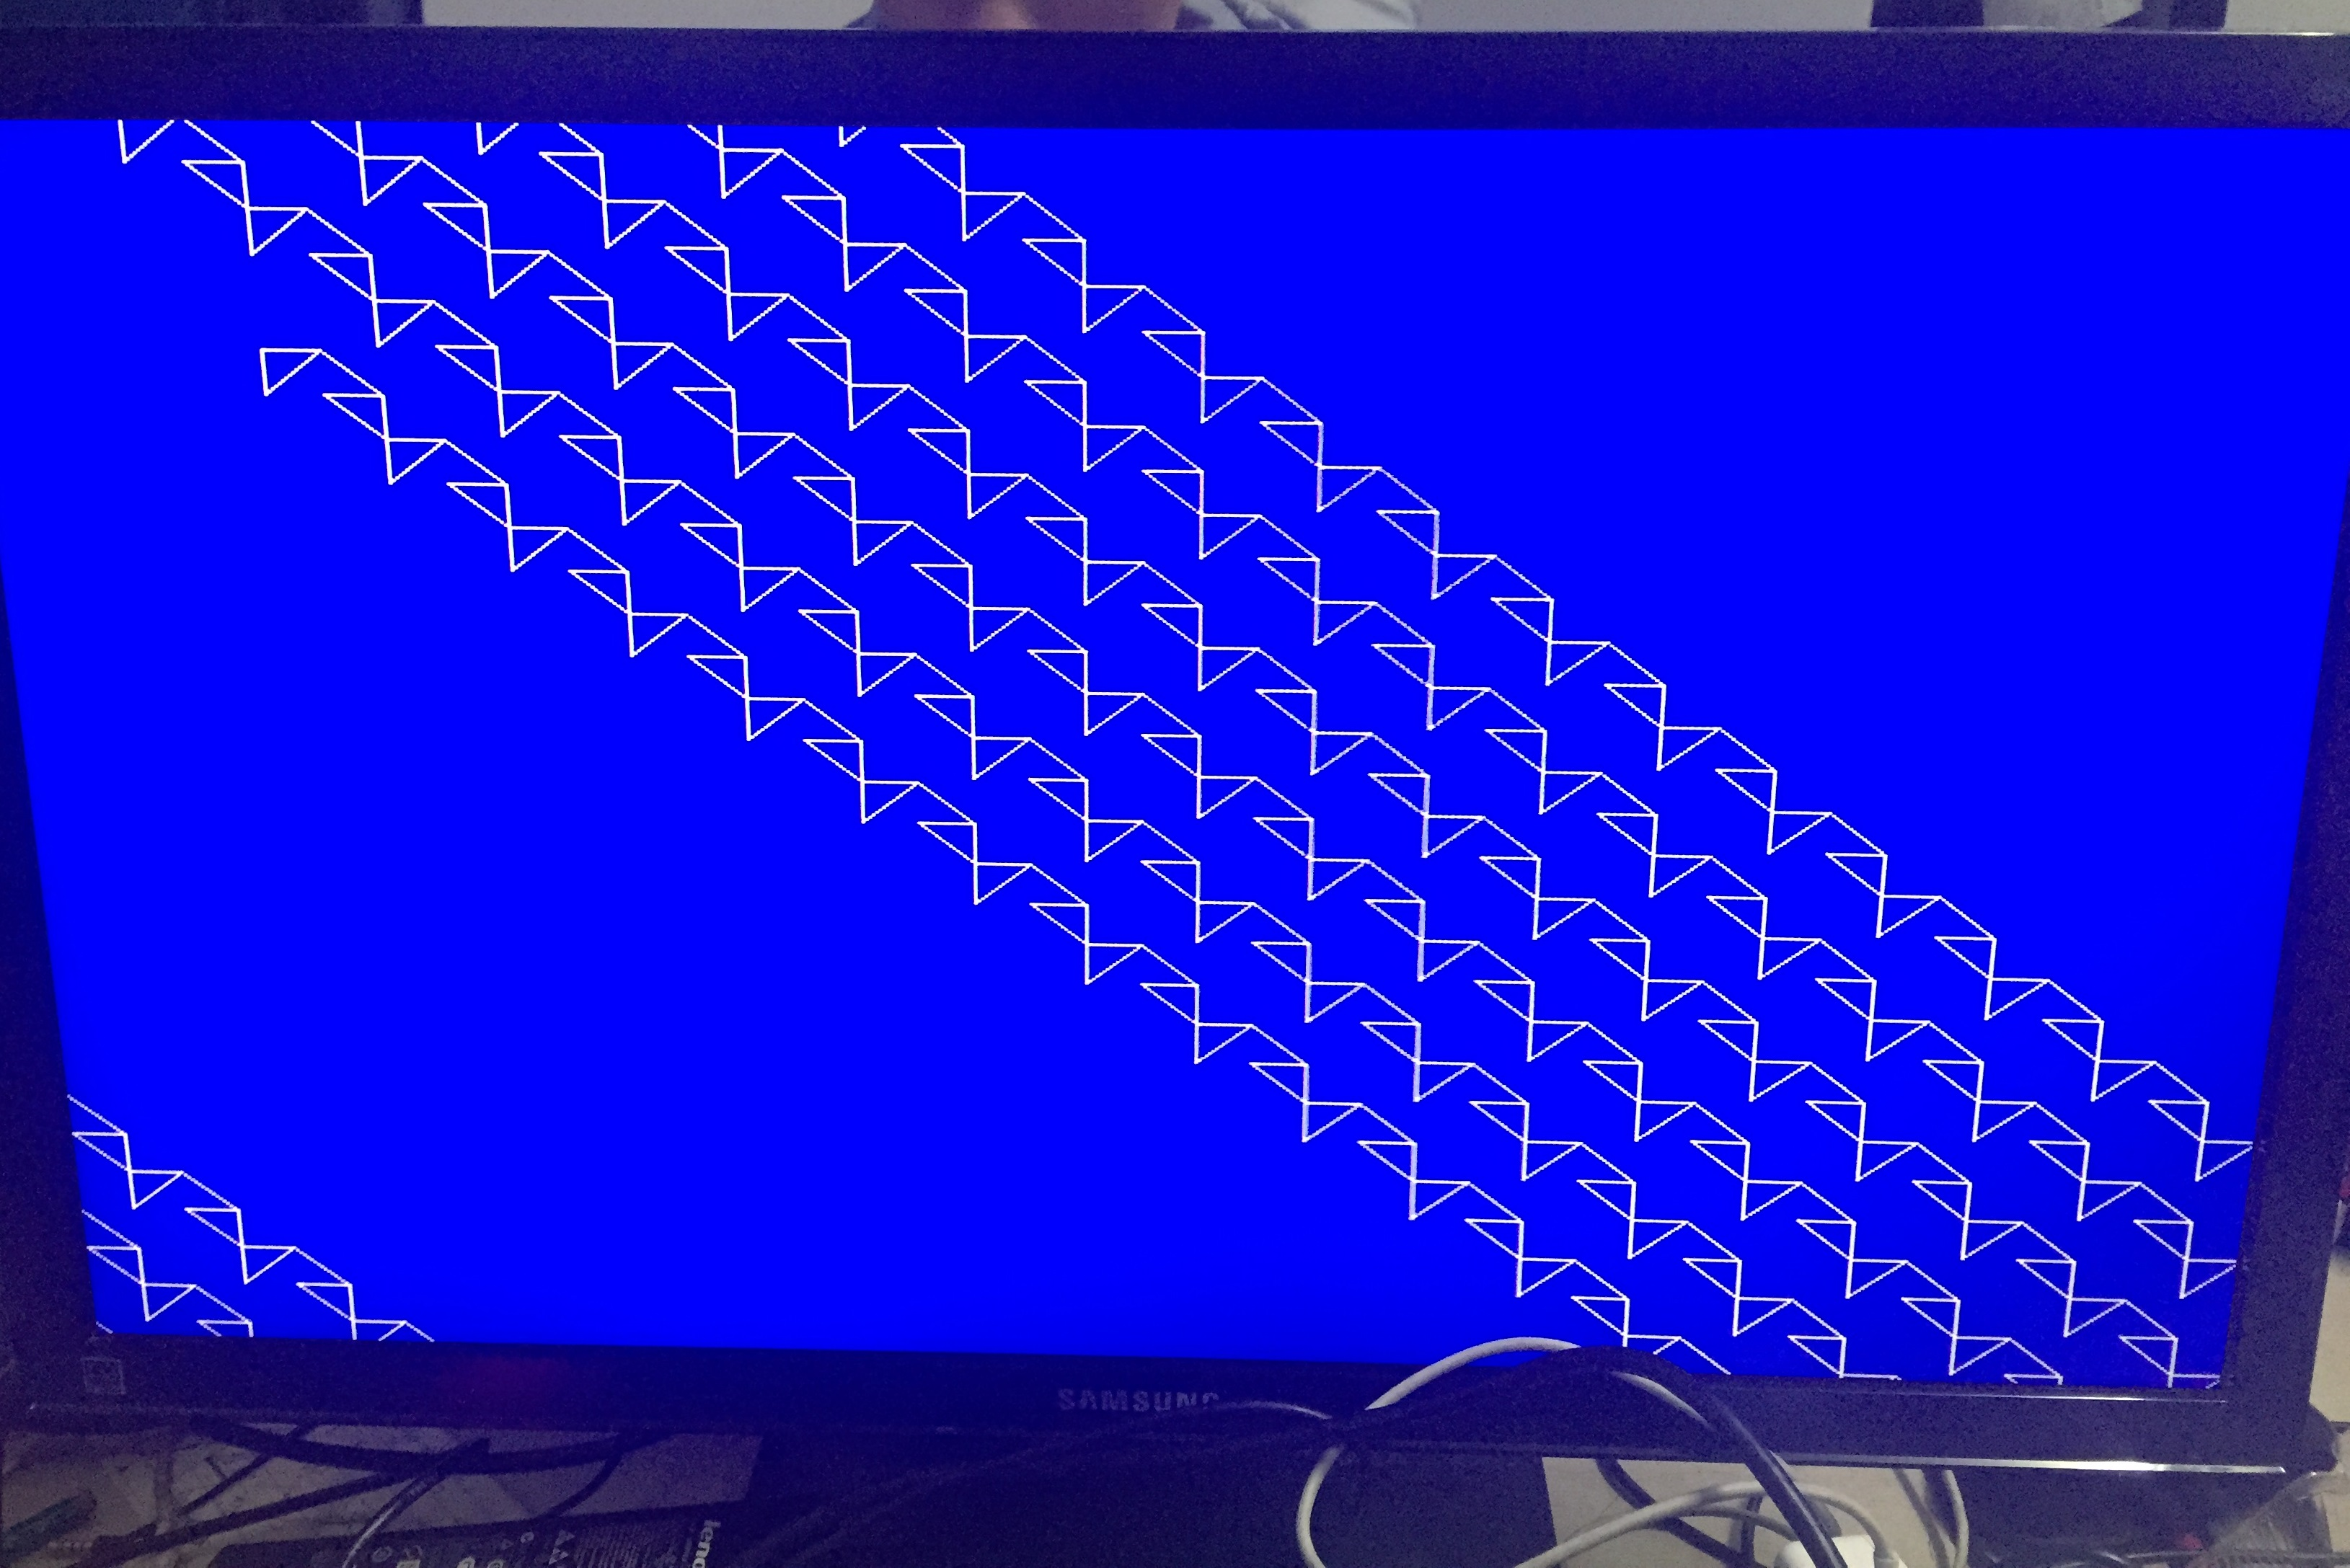
\includegraphics[width=13cm]{image/extension/tri.JPG}
    \fcaption{漂亮的三角形阵}\label{fig:tri}
\end{center}

屏幕为像素映射。我们在片内开了一块等同于屏幕可显示像素数目大小的RAM作为我们的显存(使用ISE的IP核)。我们只需修改显存即可改变屏幕上的内容,由于片内存储空间不大,所以只能显示蓝白两色。

像素映射为我们的计算机增添了\textbf{通用性}。

\subsubsection{键盘}

\begin{center}
    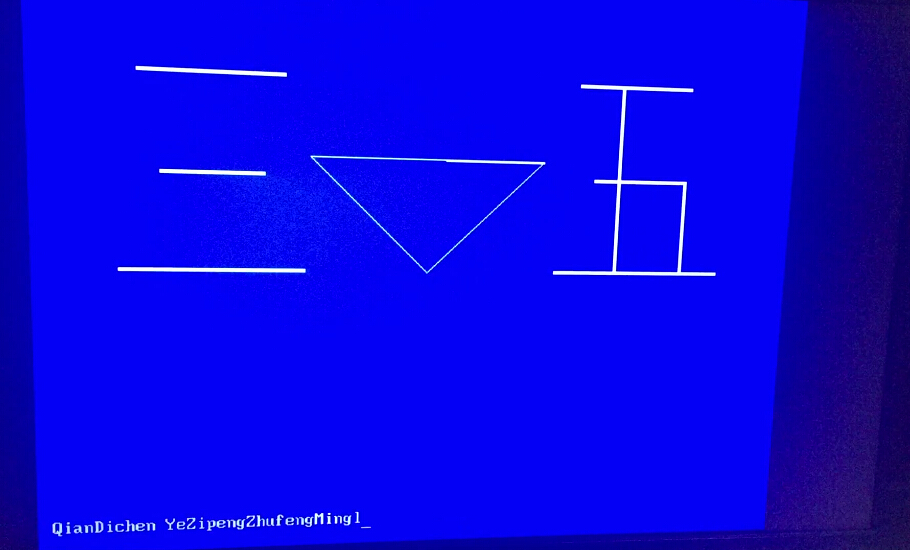
\includegraphics[width=13cm]{image/extension/35.JPG}
    \fcaption{软件中断和硬件中断的结合}\label{fig:35}
\end{center}

键盘拥有2个队列:一个叫做键盘队列(FIFO1),给硬件中断;一个叫做软中断队列(FIFO2),给软件中断。键盘输入一个字符,由硬件转译成ASCII码输送给键盘队列,当队列非空并且当时不在执行中断时,发送一个硬件中断信号,执行硬件中断。由硬件中断负责把信息转译到软中断队列。

我们使用FIFO实现了软件的缓冲区,每当回车键输入的时候,硬件中断将键盘输入的值一次性发送到软件的缓冲区,软件通过缓冲区读取字符。

\begin{enumerate}
    \item 实现$0 \thicksim 9$,$a \thicksim z$,退格键,空格键,回车键。硬件将其转化为ASCII码传入键盘队列。
    \item 实现SHIFT组合键,可以发送大写的字母,以及$0 \thicksim 9$上方的特殊字符。
    \item 手写实现键盘队列(长度为8),软中断队列(长度为16)。
\end{enumerate}

\subsubsection{硬件中断}

硬件中断是结合键盘和中央控制器实现的。每当键盘被按下,硬件中断被触发,我们会等待MEM,和WB段执行完,清空ID和ALU段。之后记录返回PC,改变PC到中断处理程序。

\subsection{细节}

\subsubsection{VGA像素映射的屏幕}

我们将大小为$640 \times 480$的整个屏幕映射到我们的显存上,我们用1位(0或1)来表示颜色,所以我们的显存空间总共为19位。

我们的显存使用的是ISE自带的IP核,由于片内存储空间仅稍大于屏幕的可显示像素数目,我们只映射2种颜色。我们的RAM是读写端口分开的,由CPU进行写数据,由VGA控制器读出数据显示到屏幕上。

VGA控制器,我们使用了上学期老师发给我们的VGA扫屏代码,我们在其之上进行修改。由于我们的显存只够显示两种颜色(蓝色和白色),我们用0表示蓝色,1表示白色,扫屏的时候通过判断值来给RGB的线赋值。这样我们即可从我们的显存中读出屏幕的值。

CPU通过总线来写显存。由于16位的字长不足以表示整个屏幕,我们使用2个字(BF08和BF09)来向显存控制器写一个像素点,第一个字表示地址的高16位,第二个字包括地址的地位和写入的数据的RGB(这里的RGB仅仅是留作对软件的接口,由于我们只能显示2种颜色,所以我们只用1位)。

由于对于我们的这种表示来说,写一个模式(一个字母或者一个图形)对软件的要求极高,我们的工作有一部分也体现在软件上。这体现了我们的硬件的通用性,也考验我们硬件的鲁棒性。

\subsubsection{键盘与中断队列}

键盘的控制器是由上学期老师发的键盘代码修改而成的。

我们的键盘控制器能把通码转成ASCII码,滤去键盘不停发送的通码,直到接收到断码为止,也就是说我们的键盘不会导致失误。除此以外,我们支持组合键(SHIFT + 按键可以产生大写的ASCII码),空格键,回车键,退格键······

键盘队列和软中断队列都是由我们自己实现。

这个队列是我们定义的一个模块,有2个端口,一个端口用于入队(写队列),一个端口用于出队(读队列)。每个端口都有各自的时钟(异步读写)和各自的使能端(如果不使能则队列保持不变)。队列内使用触发器存储数据,使用两个计数器来计数,分别表示队首和队尾。如果队首等于队尾则队列为空,否则队列非空,此时中断队列会发出中断信号,中央控制器会响应中断。

入队过程由上升沿触发,出队过程也是上升沿触发。是否入队(出队)由入队(出队)使能决定。键盘队列的容量是8个字,软中断队列的容量是16个字。

\subsubsection{硬中断}

我们每次按下键盘,键盘会将通码转换成ASCII码入队。这时队列的非空信号会触发一个硬件中断(由中央控制器实现)。

此时中央控制器会响应硬件中断,这是一个复杂的过程,整个流程分为如下几步:

\begin{enumerate}
    \item 锁住PC的写使能;
    \item 存下EPC;
    \item 清空流水线;
    \item 跳转到中断处理程序;
    \item 执行中断;
    \item 中断返回。
\end{enumerate}

我们详细说明如何清空流水线以及如何中断返回。

\textbf{确定EPC:}我们会先检查ID/ALU阶段寄存器的PC值是否为全0,如果不全0,我们将选择它。否则选择IF/ID段的PC值。为什么这样取呢?因为ID/ALU段可能是气泡,如果全0肯定是气泡,我们不能使用它。而我们整个流水线中不可能有连续2个气泡存在,所以选择IF/ID是安全的。

\textbf{清空流水线:}由于我们有分支预测,有插气泡的可能,我们认为流水线全部清空是不合适的。因为这时如果有分支预测错误,将不能复原。我们认为让流水线流完也是不合适的,此时PC的使能被锁住,如果有跳转将不能正常跳转。我们选择了一个折衷的方法,也是MIPS提倡的方法,把MEM和WB段的指令执行完,而ID和ALU段的指令清空。这样在我们的架构下不会产生冲突,中断得以正常进行。

\textbf{中断返回:}我们新增了一条\texttt{ERET}指令,代码是FFFF ,这条指令是中断执行程序的特权指令,只有在中断正在执行的时候才有效。这条指令会相当于一条\texttt{B EPC} ,表明中断执行结束,需要继续执行指令。

\subsubsection{软中断}
由软件实现,其过程需要等待硬中断的触发以及处理,通过硬中断把键盘队列中的数据转移到软中断队列中,软中断得以结束。

\section{软件}

\subsection{针对我们像素映射实现的接口}

\begin{enumerate}
    \item 给定坐标画一个点
    \item 给定起始点,长度,类型(总共8个类型,每45度角为一类)画一条细线段
    \item 给定起始点,长度,类型(同上),粗细,画一条粗线段
    \item 给定直角顶点,大小,类型(总共8个类型,每45度角为一类)画一个等腰直角三角形
    \item 从数据RAM中读取一个形状(用于实现字符集,比如汉字或是ASCII码)
\end{enumerate}

\subsection{针对键盘实现的硬件中断和软件中断的中断程序}

\subsubsection{硬件中断}

\begin{enumerate}
    \item 从键盘输入队列中取出一个ASCII码输出到串口
    \item 从键盘输入队列中取出一个ASCII码输入到软中断队列
    \item 从键盘输入队列中取出一个ASCII码,通过调用字符显示的函数显示到屏幕
    \item 实现退格键
\end{enumerate}

\subsubsection{软件中断}

该程序类似于C语言的库函数\texttt{scanf},支持char和int数据类型。其具体功能如下:

\begin{enumerate}
    \item 从软件中断队列中读取一个ASCII码;
    \item 从软件中断队列中读取一串数字,直到空格,并解析成一个INT;
    \item (暂未完成)完成一个画图程序,读入画图指令,解析成参数,传给画图函数实现画图的功能,由于时间紧张,汇编代码(1000+行)已经完成,然后没有调试完全,还不能工作。
\end{enumerate}

\subsection{定制的Term}

老师提供的Term只支持基础指令,而我们需要调试也需要使用扩展的指令。故在原有Term的基础上修改而成。

\begin{center}
    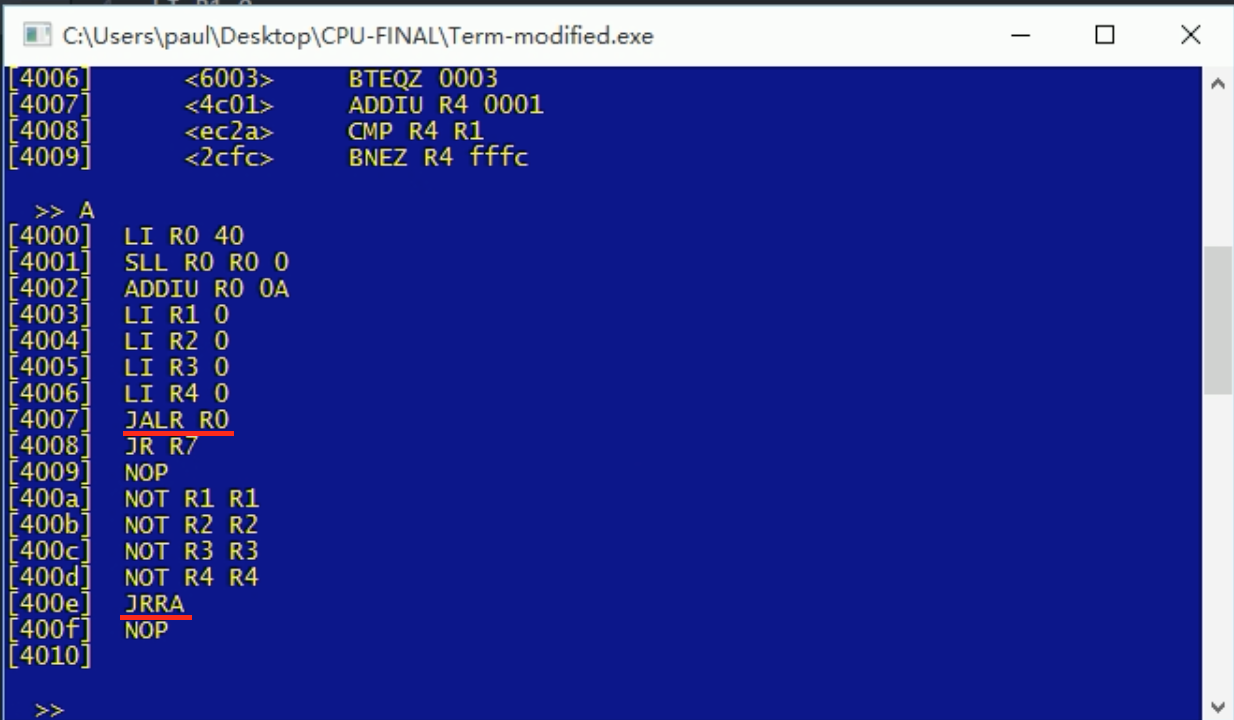
\includegraphics[width=13cm]{image/extension/term}
    \fcaption{扩展的Term}\label{fig:term}
\end{center}

我们自己的Term具备老师的Term的全部功能,除此以外,我们为它增添了新的特性,包括:

\begin{enumerate}
    \item 可以识别拓展的5条指令,包括\texttt{NOT,BTNEZ,SLT,JALR,JRRA};
    \item 可以向RAM中写入拓展的5条指令,包括\texttt{NOT,BTNEZ,SLT,JALR,JRRA};
    \item 中断的支持,对\texttt{ERET}的写入。
\end{enumerate}

实现这个Term的过程并不难,因为老师提供了Term的源码,我们只需要在指令列表中增加新指令对应的操作码以及各个操作数的位置即可。
